\section*{Reproducibility Summary}

\subsection*{Scope of Reproducibility}

The authors introduce a novel approach to analyze Generative Adversarial Networks (GANs) and create interpretable controls for image manipulation and synthesis. This is done by identifying important latent directions based on Principal Component Analysis (PCA) applied either in the latent space or the feature space. We aim to validate the claims and reproduce the results of the original paper.

\subsection*{Methodology}

The code that was provided by the authors in Pytorch was reimplemented in \textbf{Tensorflow 1.x} for the pretrained StyleGAN and StyleGAN2 architectures. This was done with the help of the APIs provided by the original authors of these models.
\\
The experiments were run on a laptop with an Intel(R) Core(TM) i7-8750H CPU @ 2.20GHz processor, 16GB RAM, NVIDIA GeForce GTX 1060 with Max-Q Design (6GB VRAM) GPU, and Ubuntu 18.04.5 LTS.

\subsection*{Results}

We were able to reproduce the results and verify the claims made by the authors for the StyleGAN and StyleGAN2 models by recreating the modified images, given the seed and other configuration parameters.
Additionally, we also perform our own experiments to identify new edits and extend the truncation trick to images generated using StyleGAN.

\subsection*{What was easy}

The paper provides detailed explanations for the different mathematical concepts that were involved in the proposed method. This, augmented with a well-structured and documented code repository, allowed us to understand the major ideas in a relatively short period of time. Running the experiments using the original codebase was straightforward and highly efficient as well, as the authors have taken additional steps to employ batch processing wherever possible.

\subsection*{What was difficult}

Originally we were attempting to recreate identical images with zero delta in the RGB values. However, due to differences in the random number generators between PyTorch-CPU, PyTorch-GPU and Numpy, the random values were not the same even with the same seed. This resulted in minute differences in the background artifacts of the generated images. Additionally, there is a lack of open source Tensorflow 1.x APIs to access the intermediate layers of the BigGAN model. Due to time constraints, we were unable to implement these accessors and verify the images that the authors of GANSpace created using BigGAN.

\subsection*{Communication with original authors}

While conducting our experiments, we did not contact the original authors. The paper and codebase were organized well and aided us in effectively reproducing and validating the authors' claims.

\newpage

\section{Introduction}

A Generative Adversarial Network (GAN)\cite{gan} is a machine learning framework where two neural networks, the discriminator and the generator, compete with each other in a zero-sum game. The generator tries to trick the discriminator into believing that artificially generated samples belong to real data.

GANs have proven to be powerful image synthesis tools and are capable of producing high quality images. However, they provide little control over the features of the generated image. Existing solutions\cite{supervised} that add user control over the generated images require expensive supervised training on latent vectors.

GANSpace\cite{GANSpace} proposes a simple technique to discover interpretable GAN controls in an unsupervised manner. This is done by identifying important latent directions based on Principal Component Analysis (PCA) applied either on the latent space or the feature space. The author's experiments on StyleGAN\cite{stylegan}, StyleGAN2\cite{stylegan2} and BigGAN512-deep\cite{biggan} demonstrate that layer-wise decomposition of PCA directions leads to many interpretable controls, which affect both low and high level attributes of the output image.


\section{Scope of reproducibility}
\label{claims}


For our reproduction study, we aim to validate the effectiveness of the proposed technique in offering powerful interpretable controls on the output images in an unsupervised manner.

The following claims of the paper have been verified and tested successfully:
\begin{itemize}[noitemsep]
    \item PCA can be used to highlight important directions in the GAN's latent space.
    \item The GAN's output can be controlled easily in an unsupervised fashion.
    \item The earlier components control the higher-level aspects of an image, while the later directions primarily affect the minute details.
    \item Random directions do not yield meaningful decompositions as compared to the principal components identified using PCA.
\end{itemize}


\section{Methodology}

The principal components\cite{hotelling1933analysis} of a collection of points in real coordinate space are a sequence of $p$ unit vectors, where the $i^{th}$ vector is a direction of the line that best fits the data while being orthogonal to the remaining $i-1$ vectors. Principal Component Analysis (PCA) is an unsupervised algorithm used to compute the principal components and perform a change of basis of the data using one or more of the computed components, increasing the interpretability of the data while minimizing its information loss\cite{jolliffe2016principal}. It is commonly used in exploratory data analysis and for dimensionality reduction when dealing with high-dimensional noisy data. The authors of GANSpace propose a technique for identifying interpretable controls in an unsupervised fashion on pretrained GANs using PCA. Specifically, they show that layer-wise perturbations along the principal components generated using PCA on the latent space of StyleGAN based networks can be used to generate human-interpretable transformations on the synthesized images.

Mathematically, a GAN can be expressed as a neural network $G(\textbf{z})$ that generates an image $I: \textbf{z} \sim p(\textbf{z}), I = G(\textbf{z})$. Here, $p(\textbf{z})$ is a probability distribution from which the latent vector $\textbf{z}$ is sampled. The network $G(\textbf{z})$ can be further decomposed into $L$ intermediate layers $G_1\ldots G_L$. In the StyleGAN/StyleGAN2 models, the input to the first layer is a constant $\textbf{y}_0$. The output and input to the remaining layers is computed as:

\begin{equation}
  y_i = G_i(y_{i-1}, \mathbf{w}),\text{ where }\mathbf{w} = M(\mathbf{z})
\end{equation}

$M$ is a an $8$-layer multilayer perceptron which is a non-linear function of $\textbf{z}$. The number of layers $L$ depends on the resolution of the generated image. At each layer, the generated image is upsampled by a factor of $2$.

\begin{figure}[H]
  \centering
  \includegraphics[scale=0.25]{figs/stylegan.png}
  \caption{Architecture of StyleGAN\cite{stylegan}}
  \label{fig:stylegan}
\end{figure}

\begin{figure}[H]
  \centering
  \includegraphics[width=\textwidth]{figs/stylegan2.png}
  \caption{Architecture of StyleGAN2\cite{stylegan2}}
  \label{fig:stylegan2}
\end{figure}

The images generated by StyleGAN and StyleGAN2 can be controlled by identifying the principal axes of $p(\textbf{w})$, which is the probability distribution of the output of the mapping network $M$. First, we sample $N$ latent vectors $\textbf{z}_{1:N}$ and compute the corresponding $\textbf{w}_{i} = M(\textbf{z}_{i})$. The PCA of these $\textbf{w}_{1:N}$ values gives us the basis $\textbf{V}$ for $\mathcal{W}$. The output attributes of a new image given by $\textbf{w}$ can then be controlled by varying the PCA coordinates of \textbf{x} before feeding them into the synthesis network:

\begin{equation}
    \mathbf{w'} = \mathbf{w} + \mathbf{Vx}
\end{equation}

Each entry $x_{k}$ of \textbf{x} is a separate control parameter which can be modified to update the desired attributes of the output image.

We follow the same notation used by the authors to denote edit directions in this report. $E(\textbf{v}_{i}, j-k)$ means moving along component $\textbf{v}_{i}$ from layers $j$ to $k$. Identifying specific edits, for example "changing the color of a car", is done via exploratory analysis using a trial-and-error method. The authors have created a GUI-based application for this purpose.

\subsection{Model descriptions}

We use NVIDIA's official implementation of StyleGAN\footnote{\url{https://github.com/NVlabs/stylegan}} and StyleGAN2\footnote{\url{https://github.com/NVlabs/stylegan2}} models.
The original code uses a PyTorch/NumPy implementation of StyleGAN and StyleGAN2 which creates a PyTorch model and copies the weights from NVLabs' implementations which are in Tensorflow. However, we directly use the NVLabs' APIs with NumPy and make changes to the official GANSpace codebase to support the same.

\subsection{Datasets}

The experiments in the paper were performed using the FFHQ, LSUN Car, CelebA-HQ, Wikiart, Horse and Cat datasets. The official Tensorflow implementation of StyleGAN contains links to download pretrained models on FFHQ, LSUN Car, Wikiart, Horse and Cat. The models trained on Wikiart were downloaded from awesome-pretrained-stylegan\footnote{\url{https://github.com/justinpinkney/awesome-pretrained-stylegan}}.

In addition to the datasets used by the authors, we also perform our own experiments on the Beetles dataset which was downloaded from awesome-pretrained-stylegan2\footnote{\url{https://github.com/justinpinkney/awesome-pretrained-stylegan2}}.


\subsection{Experimental setup}

All the experiments were conducted on a laptop with an Intel(R) Core(TM) i7-8750H CPU @ 2.20GHz processor, 16GB RAM, NVIDIA GeForce GTX 1060 with Max-Q Design (6GB VRAM) GPU, and Ubuntu 18.04.5 LTS. The generated images from our experiments were evaluated visually to determine whether the edits were working as expected.

\section{Results}

We were able to reproduce the results and verify the claims (mentioned in Section \ref{claims}) made by the authors for the StyleGAN and StyleGAN2 models by recreating the modified images, given the configuration parameters. Additionally, we also perform our own experiments to provide additional results that validate the effectiveness of the technique employed by GANSpace.


\subsection{Effectiveness of PCA}

\begin{figure}[H]
    \centering
    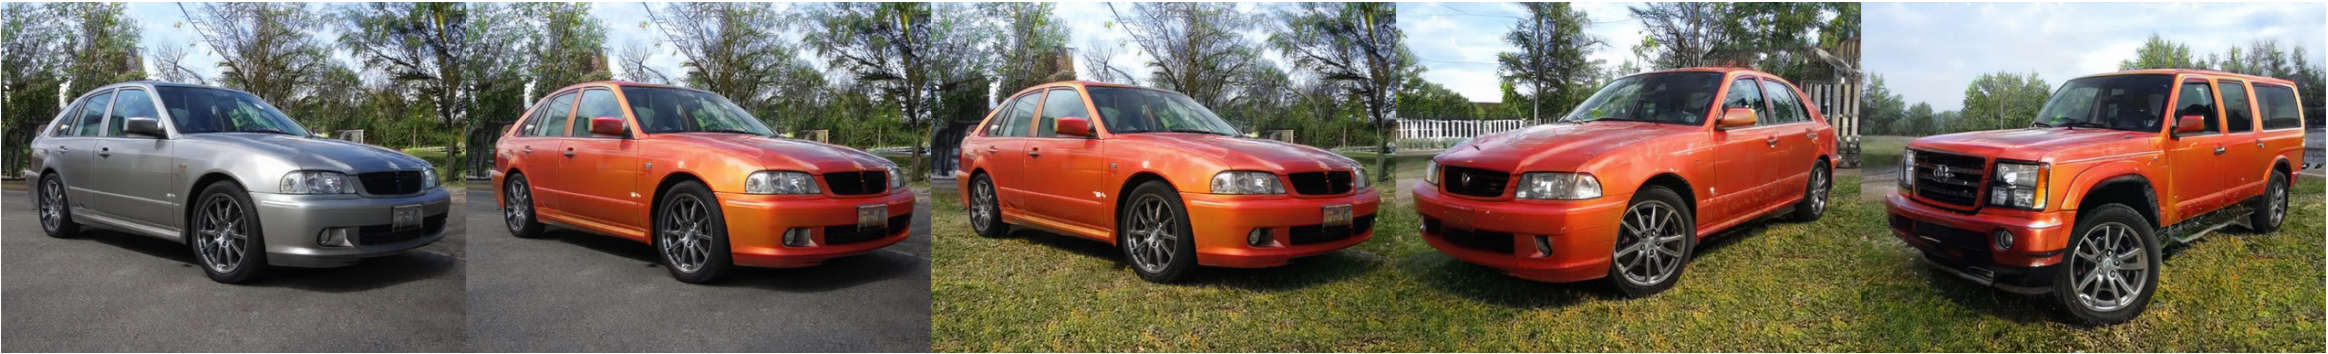
\includegraphics[width=\textwidth]{figs/figure1_StyleGAN2_cars.png}
    \caption{Sequences of image edits performed using control discovered with StyleGAN2 cars: ``Initial Image" $\rightarrow$ ``Change Color" $\rightarrow$ ``Add Grass" $\rightarrow$ ``Rotate" $\rightarrow$ "Change Type"}
    \label{fig:cars}
\end{figure}

Figure \ref{fig:cars} highlights the effectiveness of PCA on changing the low and high level attributes of the image. We are able to control object shape, colour and pose as well as nuanced landscape attributes.

The edit directions corresponding to each of the edits are: $E(\textbf{v}_{22}, 9-10)$ ("Change Color"), $E(\textbf{v}_{11}, 9-10)$ ("Add Grass"), $E(\textbf{v}_{0}, 0-4)$ ("Rotate") and $E(\textbf{v}_{16}, 3-5)$ ("Change type").

\subsection{Unsupervised vs. Supervised methods}

\begin{figure}[H]

  \subfloat[Edit directions identified by PCA ($E(\textbf{v}_{1}, 0-1)$)]{%
    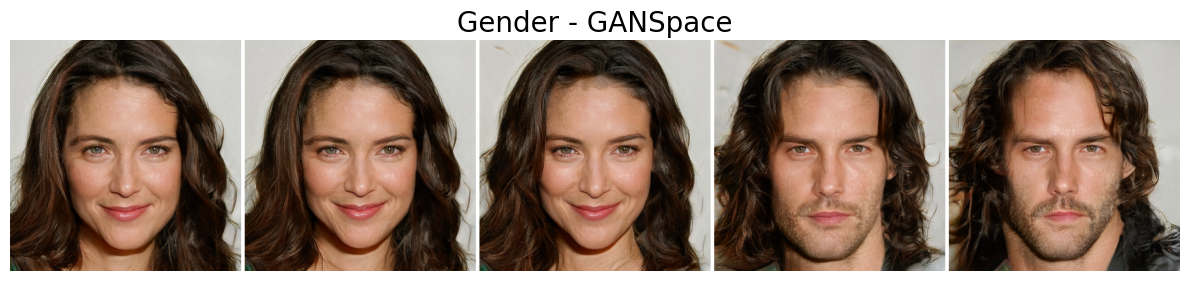
\includegraphics[clip,width=\columnwidth]{figs/figure5_Gender-GANSpace_scale=-3dot2.png}
  }

  \subfloat[Edit directions identified by supervised methods\cite{supervised}]{%
    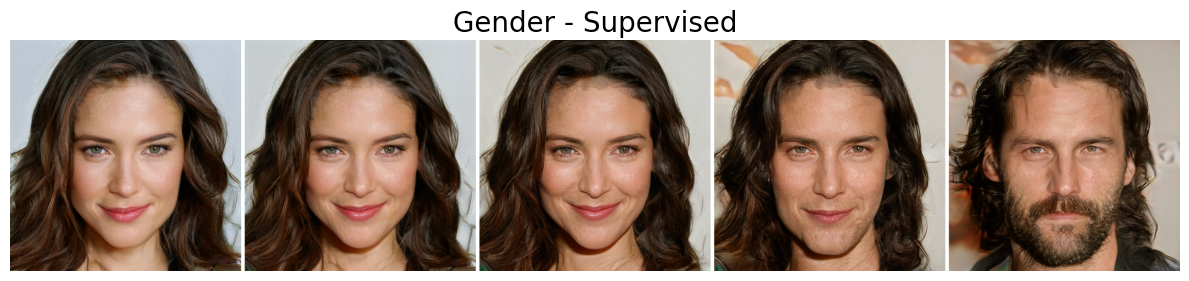
\includegraphics[clip,width=\columnwidth]{figs/figure5_Gender-Supervised_scale=1dot2.png}
  }
  
  \caption{Comparison of edits using unsupervised and supervised methods}
  \label{fig:faces}
\end{figure}

Previous methods for finding interpretable directions in GAN latent spaces require external supervision, such as labeled training images or pretrained classifiers. GANSpace, on the other hand, automatically identifies variations intrinsic to the model without supervision. This has been validated using the CelebA-HQ Faces dataset by comparing the edit directions found through PCA to those found in previous works using supervised methods.

Figure \ref{fig:faces} shows that comparable edits can be obtained in a completely unsupervised fashion. Additionally, GANSpace can be used to identify new edits which have not been previously demonstrated. Supervised methods are not viable for this task as supervising each new edit would be costly. It is also difficult to know in advance which edits are even possible in supervised approaches.

\subsection{PCA components vs. Random directions}

\begin{figure}[H]
    \centering
    \includegraphics[width=\textwidth]{figs/cats.png}
    \caption{Illustration of the significance of the principal components as compared to random directions in the intermediate latent space of StyleGAN2.}
    \label{fig:cats}
\end{figure}

The original authors claim that the earlier PCA components primarily control the geometry and other high-level aspects (pose and style), while the lower components capture minute details. Additionally, they claim that fixing and randomizing randomly-chosen directions do not yield PCA-like meaningful decompositions, thus showing the importance of identifying good directions using PCA. This has been illustrated in Figure \ref{fig:cats}, where different subsets of principal coordinates and random coordinates are randomized while keeping the latent vector constant. In Figure \ref{fig:cats}a, the first eight principal coordinates $\textbf{x}_{0:7}$ are fixed and the remaining $504$ coordinates $\textbf{x}_{8:512}$ are randomized. This changes the background and appearance of the cat while keeping the cat's pose and camera angle constant. Conversely, Figure \ref{fig:cats}b shows that fixing the last $504$ coordinates and randomizing the first eight yields images where the camera and orientation vary, but the color and appearance are held roughly constant. Figure \ref{fig:cats}c and Figure \ref{fig:cats}d shows the results of the same process applied to random directions. The images illustrate that any given $8$ directions have no distinctive effect on the output.

\subsection{Additional results not present in the original paper}

\subsubsection{New edits}

We identify new edits on the Stylegan2 Beetles dataset. Edit $E(\textbf{v}_{2}, 0-17)$, referred to as "Patterns", adds a pattern on the shell of the beetle as well as increasing the overall size of the beetle. The generated pattern varies depending on the seed used to sample $\textbf{w}$.

\begin{figure}[H]

\subfloat[Beetle generated with seed 1819967864]{%
  \includegraphics[clip,width=\columnwidth]{figs/figure7_beetles_pattern.png}%
}

\subfloat[Beetle generated with seed 1]{%
  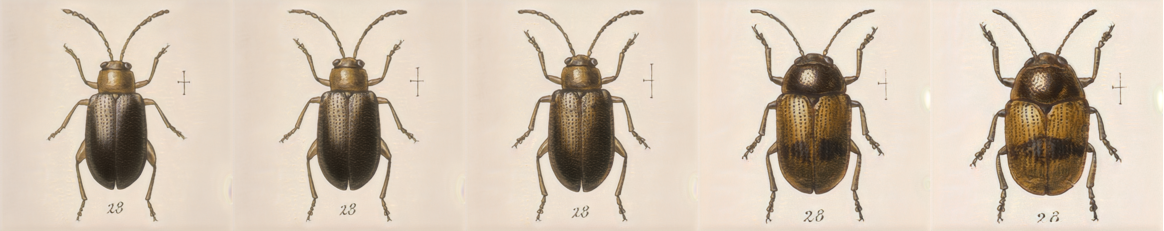
\includegraphics[clip,width=\columnwidth]{figs/figure7_different_beetle_pattern.png}%
}

\caption{"Patterns" edit applied on the output images of StyleGAN2 Beetles}

\end{figure}

\subsubsection{Truncation Trick on StyleGAN}

The "Truncation Trick" is a procedure applied to the latent vectors to improve the quality of the generated images at the expense of variety in the images. It does this by sampling the latent vectors from a truncated distribution that is closer to the average of the latent vectors sampled during training, thereby reducing the variance of the latent vectors used during inference. The authors of \cite{biggan} show that using the truncation trick improves the Fréchet Inception Distance (FID) and Inception Score (IS).

In the StyleGAN/StyleGAN2 models, the truncation trick is applied on the latent space $\textbf{w}$, which is the output of the mapping network $M$. During the training process, a running average $\textbf{w}_{avg}$ of the latents is computed. Later, the latents sampled during inference are truncated to lie close to $\textbf{w}_{avg}$. Equation~\ref{eq:2} shows the truncation process on StyleGAN/StyleGAN2 models:

\begin{equation}
    \mathbf{w'} = \mathbf{w}_{avg} + \psi (\mathbf{w} - \mathbf{w}_{avg})
    \label{eq:2}
\end{equation}

During our experiments, we noticed that the original authors use the truncation trick on images generated using StyleGAN2 to reduce the number of artifacts. However, this is not enabled for StyleGAN images. We found that enabling truncation while applying edits on StyleGAN images improved their quality as well. We demonstrate this using the Wikiart dataset through the "Head Rotation" ($E(\textbf{v}_{7}, 0-1)$) and "Simple Strokes" ($E(\textbf{v}_{9}, 8-14)$ edits. In Figure~\ref{fig:truncation_psi}, we can see that the generated faces contain less noise and artifacts when the truncation trick is used. For example, the lower half of the person's face in the "Head Rotation" image does not contain as much noise as their counterpart which does not employ the truncation trick. Here, we can also observe the change in the generated images as truncation psi is decreased a lower value of $0.25$. This truncates the sampled latents to lie very close to the average and results in images that look very similar to each other. If truncation psi is set to $0$, then according to Equation~\ref{eq:2}, we can see that the truncated latent $\textbf{w}'$ is always equal to $\textbf{w}_{avg}$.

\begin{figure}

\subfloat["Head Rotation" and "Simple Strokes" edits on StyleGAN Wikiart with truncation psi set to 0.25]{%
  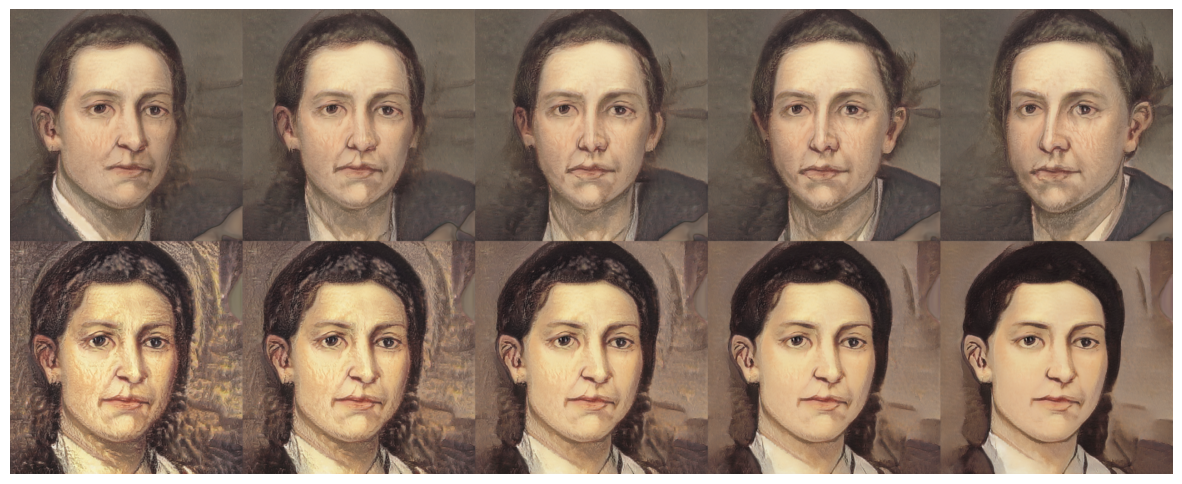
\includegraphics[clip,width=\columnwidth]{figs/wikiart_truncation_psi_0dot25.png}
}

\subfloat["Head Rotation" and "Simple Strokes" edits on StyleGAN Wikiart with truncation psi set to 0.7]{%
  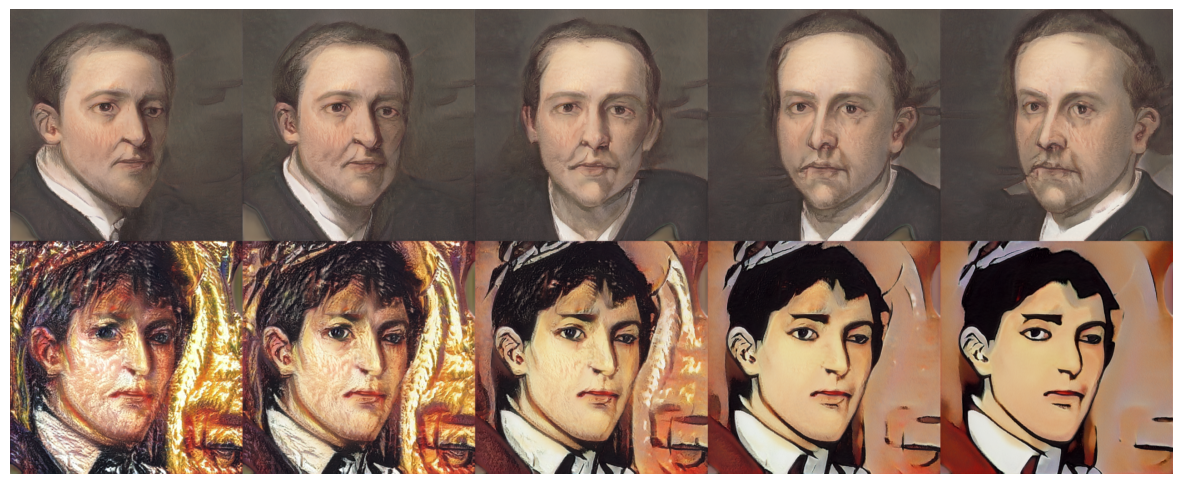
\includegraphics[clip,width=\columnwidth]{figs/wikiart_truncation_psi_0dot7.png}
}

\subfloat["Head Rotation" and "Simple Strokes" edits on StyleGAN Wikiart without truncation psi]{%
  \includegraphics[clip,width=\columnwidth]{figs/wikiart_truncation_psi_1dot0.png}%
}

\caption{Quality of images generated by StyleGAN before and after applying the "truncation trick".}
\label{fig:truncation_psi}
\end{figure}

\section{Discussion}

After performing our experiments, we feel that the results justify the claims of the paper. This is further bolstered by the fact that the proposed method worked on different datasets which were not covered by the original authors.

\subsection{What was easy}

The paper provides detailed explanations for the different mathematical concepts that were involved in the proposed method. This, augmented with a well-structured and documented code repository, allowed us to understand and verify the major ideas in a relatively short period of time. Additionally, the paper provided a lot of examples on various datasets to demonstrate exactly how their algorithm works. The authors ensured that all the figures in the paper had accompanying code to recreate them.

NVIDIA's implementation of StyleGAN and StyleGAN2 provided access to well written API's which we could integrate easily into the author's codebase.

\subsection{What was difficult}

While running our experiments, we noticed that there was a small difference in the RGB values of the recreated images. This was due to the difference in the random values generated by PyTorch-CPU, PyTorch-GPU and Numpy random number generators even when seeded with the same seed. The noise variables in the StyleGAN networks were not identical because of this. This resulted in minute differences in background artifacts of the images.

\begin{table}[H]
\centering
\begin{tabular}{cc}
\hline
Python Library & Random Number \\ \hline
PyTorch 1.3.1 (CPU)     & 0.3367                 \\
PyTorch 1.3.1 (GPU)     & 0.1940                 \\ 
Numpy 1.20.1            & 0.49671415             \\ \hline
\end{tabular}
\caption{Random values generated using different Python libraries seeded with 42}
\end{table}

We were not able to replicate the author's experiments on BigGAN512-deep due to time constraints. 

\subsection{Communication with original authors}

While conducting our experiments, we did not contact the original authors. The paper and codebase were organized well and aided us in effectively reproducing and validating the authors' claims.